\begin{figure}[!h]
\begin{center}
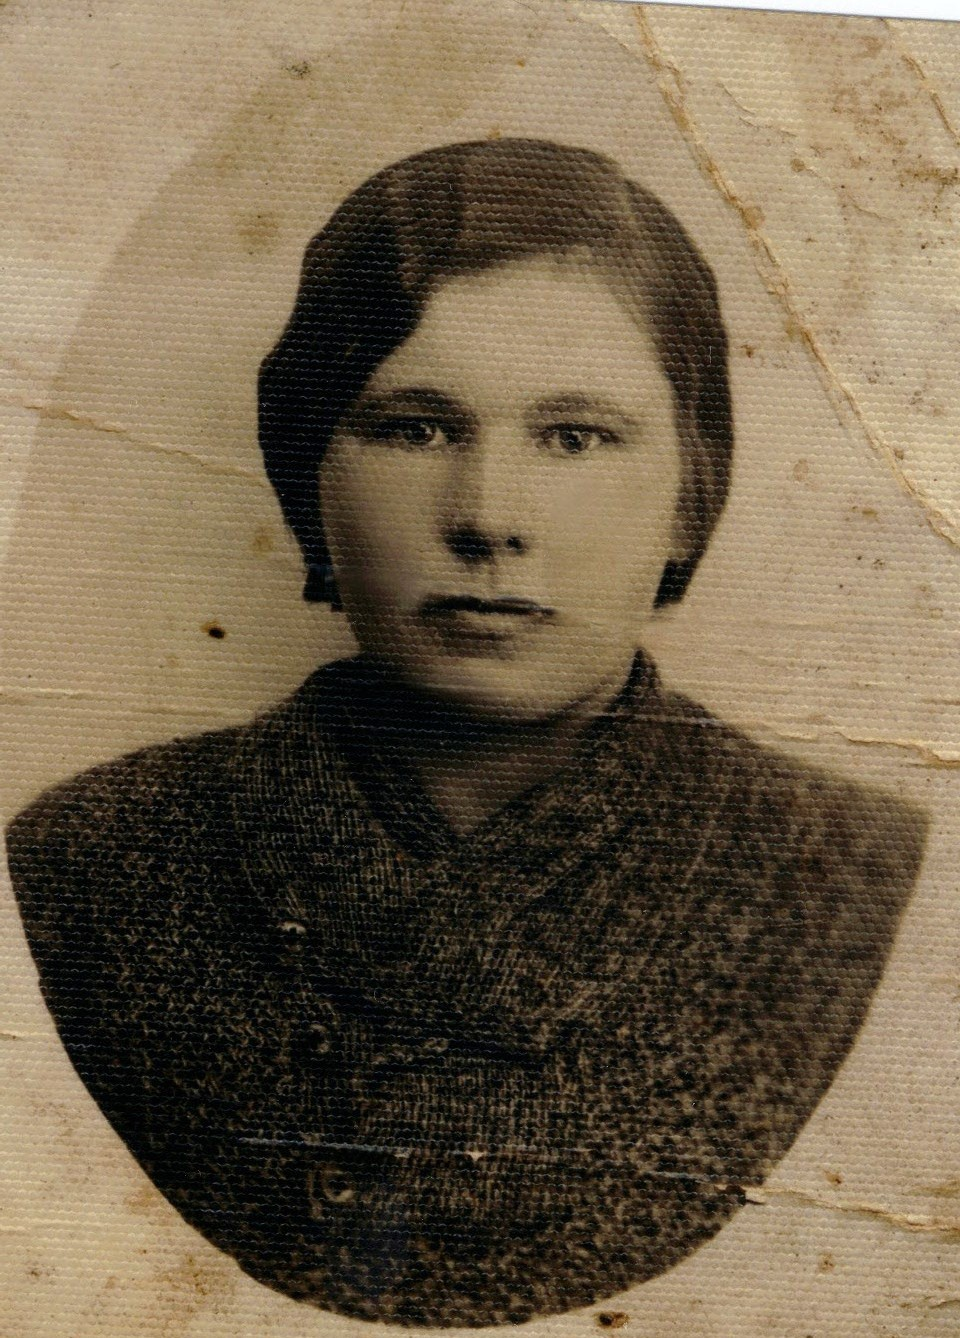
\includegraphics[width=0.4\textwidth]{zdjecia/boleslawa_glab.jpg}
\caption{Bolesława Głąb}
\label{rys:boleslawa_glab}
\end{center}
\end{figure}

Kolejnym dzieckiem Antoniny i Walentego była Bolesława Głąbówna, która przyszła na świat 28 lutego 1908 r. w Mirowie.

\begin{figure}[!h]
\begin{center}
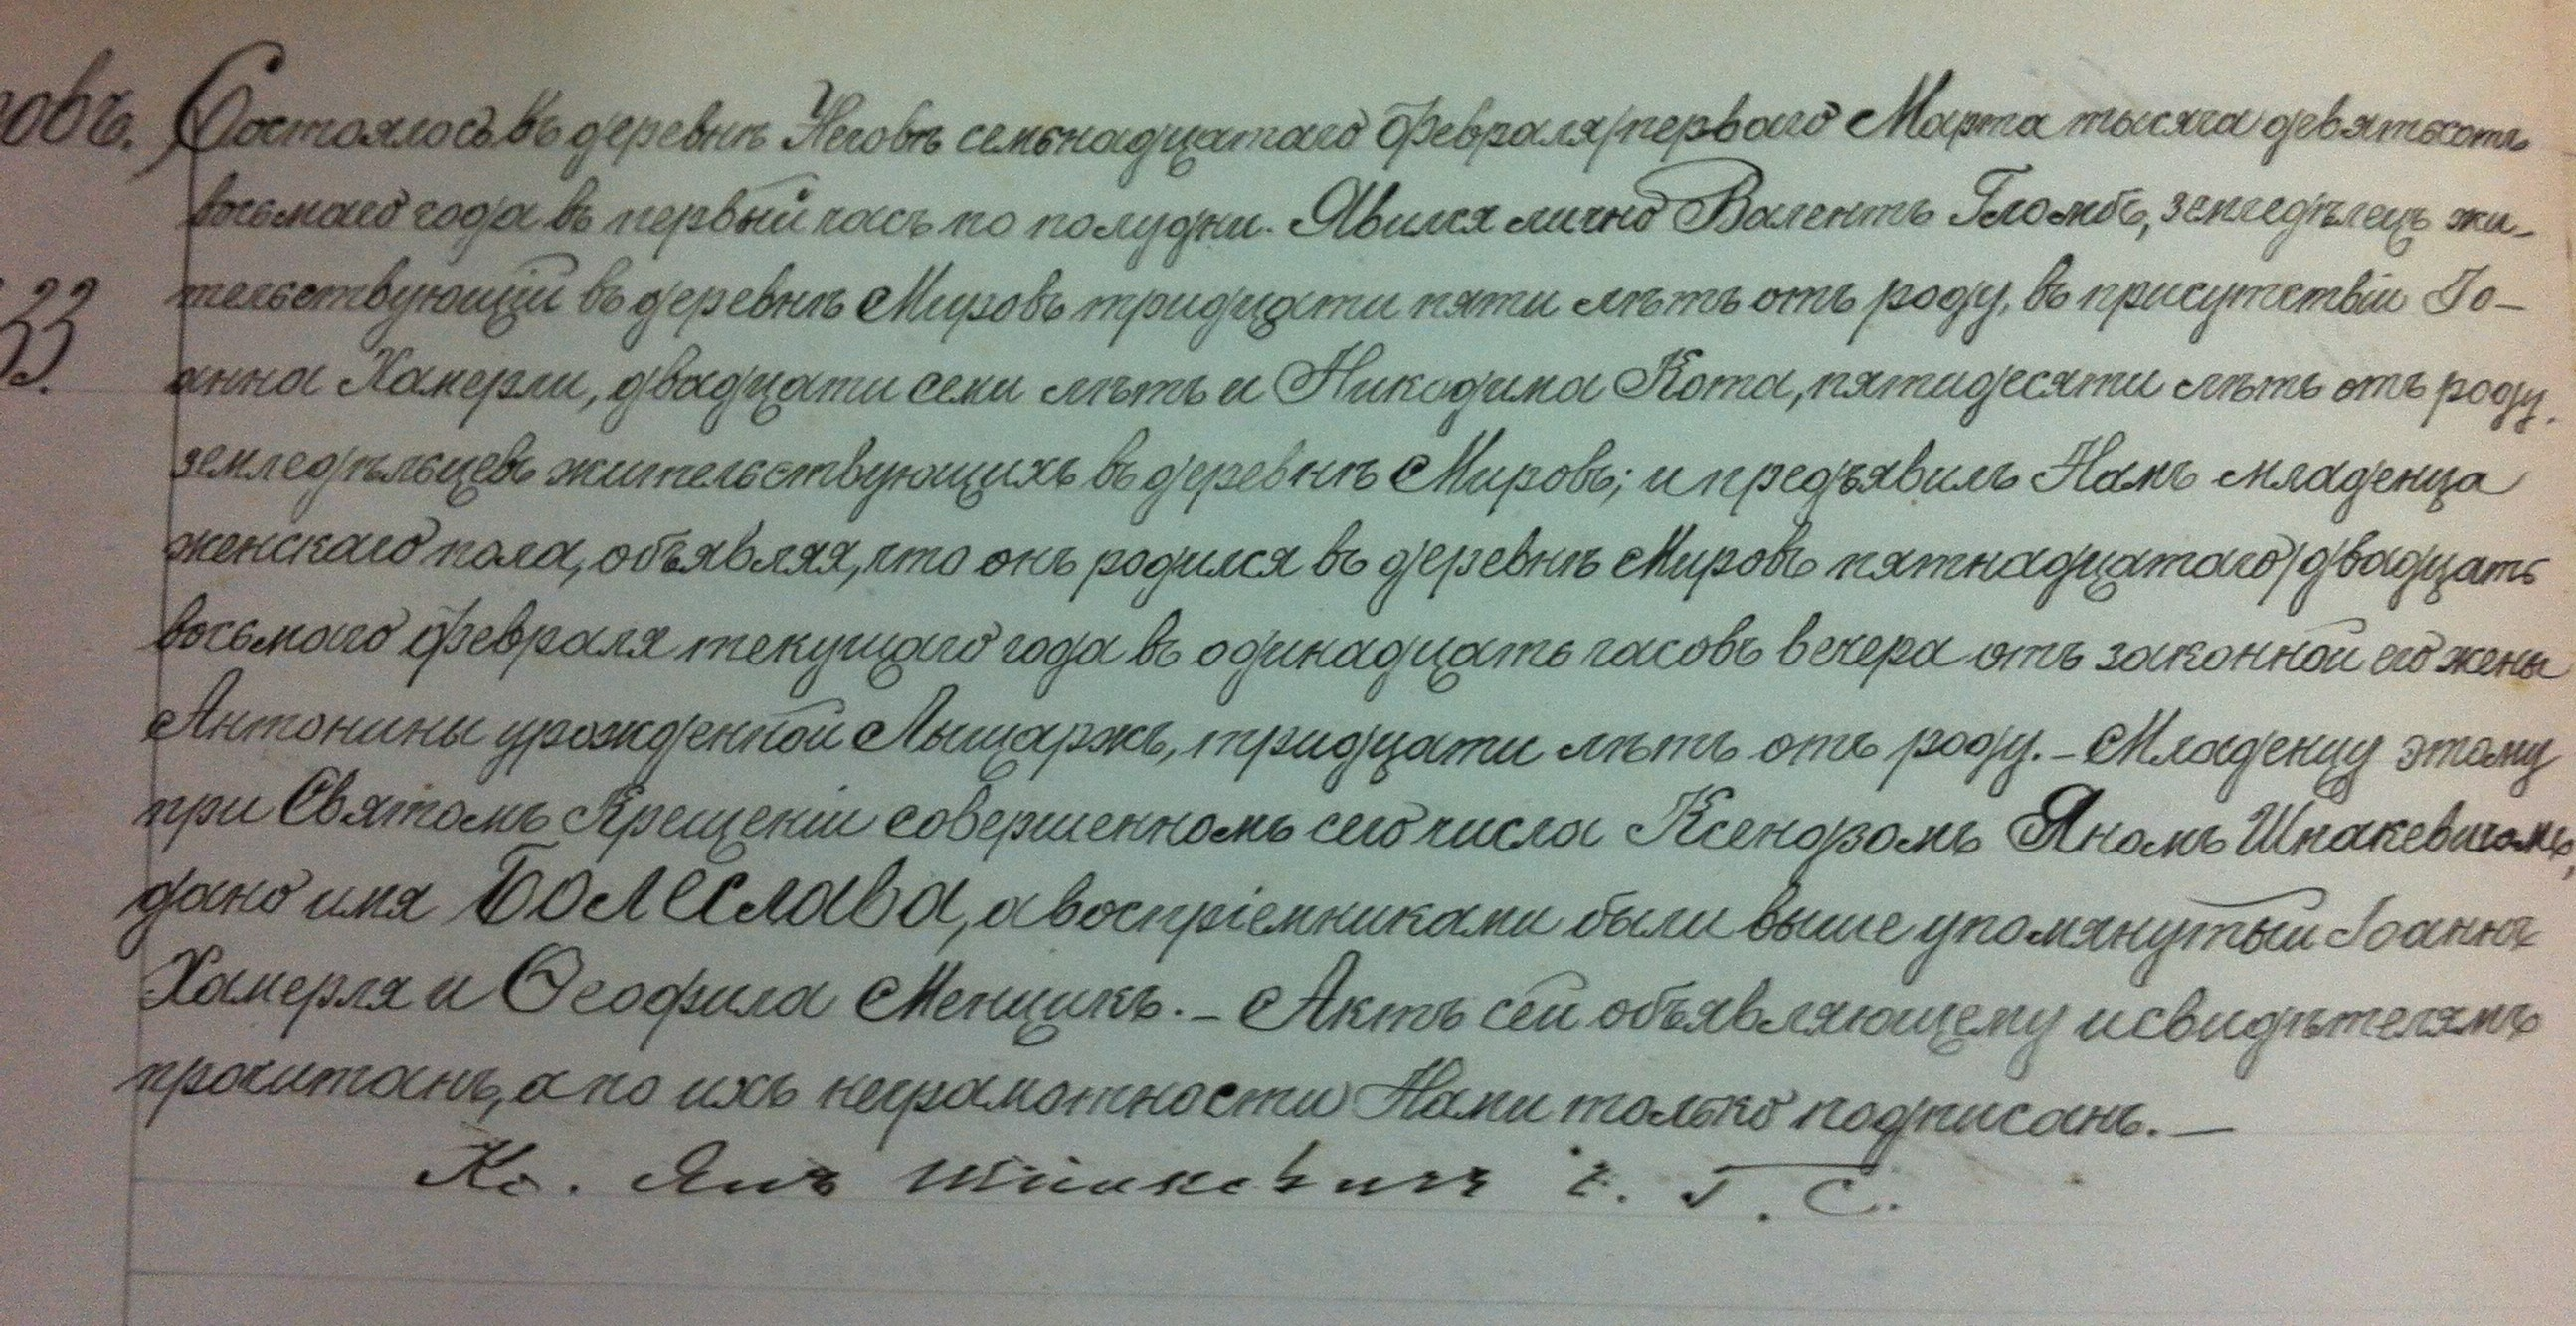
\includegraphics[width=0.8\textwidth]{zdjecia/akt_urodzenia_boleslawy_glab.jpg}
\caption{Akt urodzenia Bolesławy Głąb}
\label{rys:akt_urodzenia_boleslawy_glab}
\end{center}
\end{figure}

Wyszła ona dnia 5 IX 1932 r. w Niegowie za Bolesława Kurka (ur. 26 X 1904 r. w Mirowie, syna Józefa i Marianny z domu Dudek).

\begin{figure}[!h]
\begin{center}
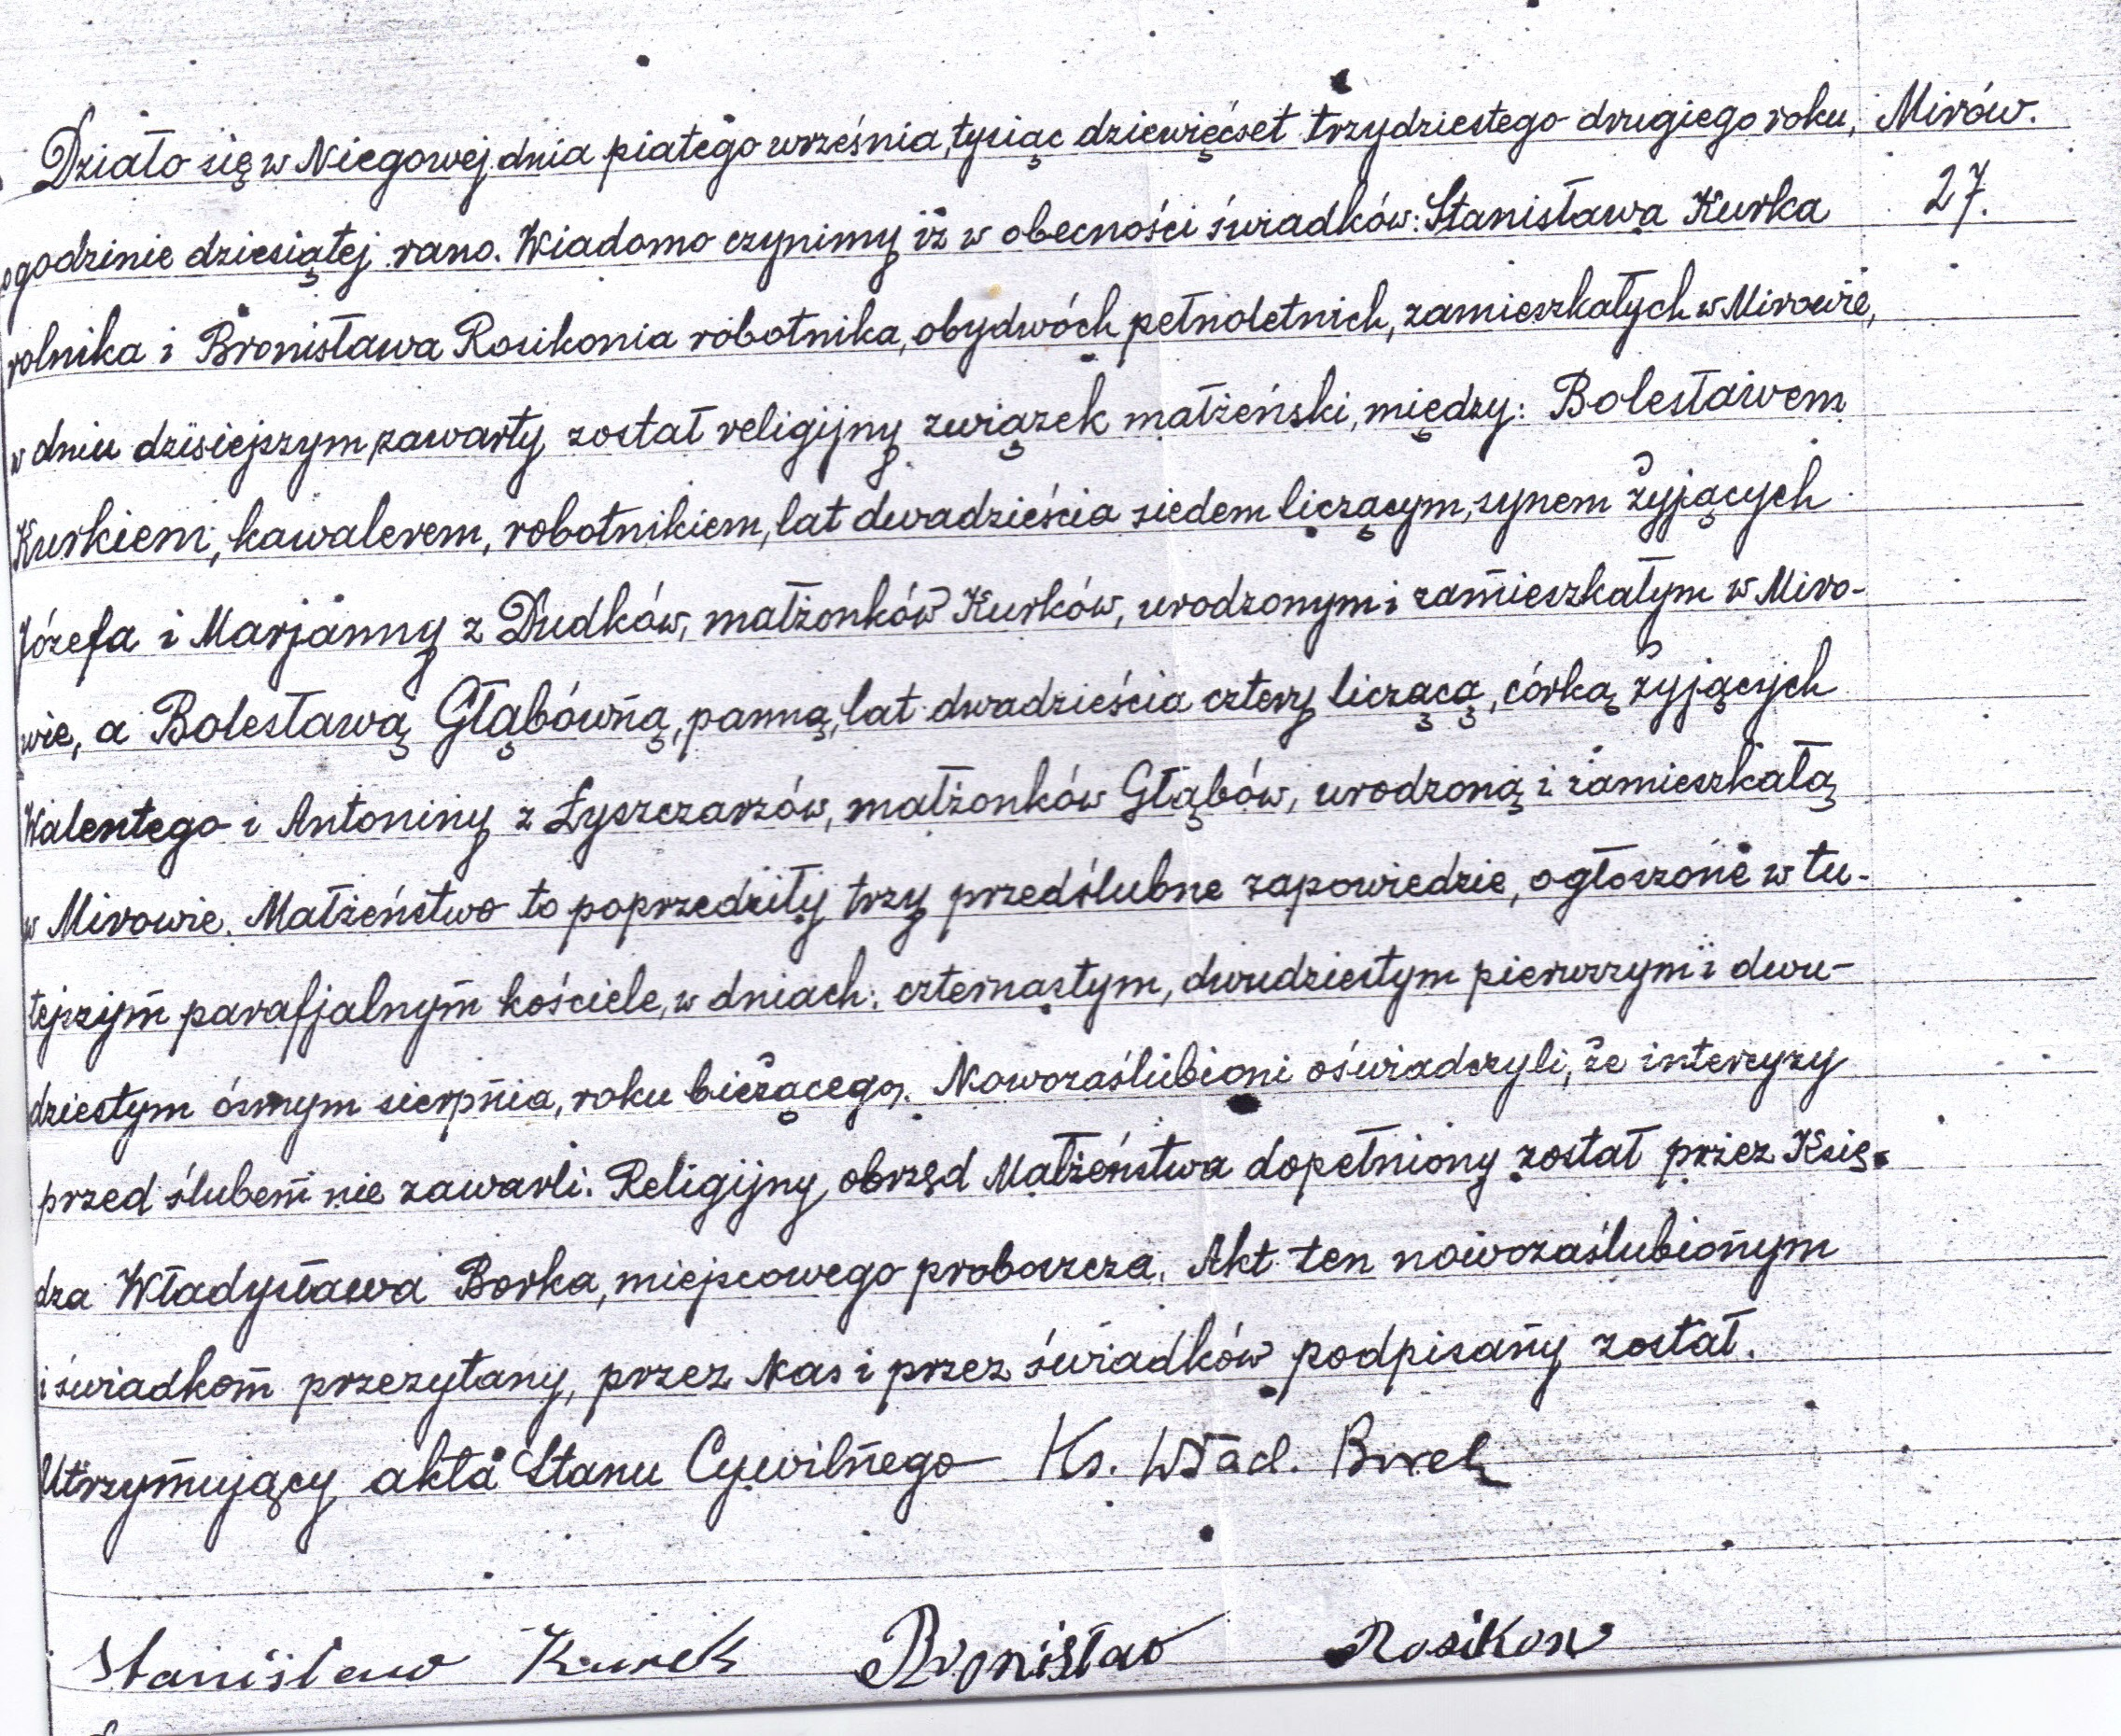
\includegraphics[width=0.8\textwidth]{zdjecia/akt_slubu_boleslawy_i_boleslawa_kurkow.jpg}
\caption{Akt ślubu Boleslawy Głąbówny z Bolesławem Kurkiem}
\label{rys:akt_slubu_boleslawy_i_boleslawa_kurkow}
\end{center}
\end{figure}

\begin{figure}[!h]
\begin{center}
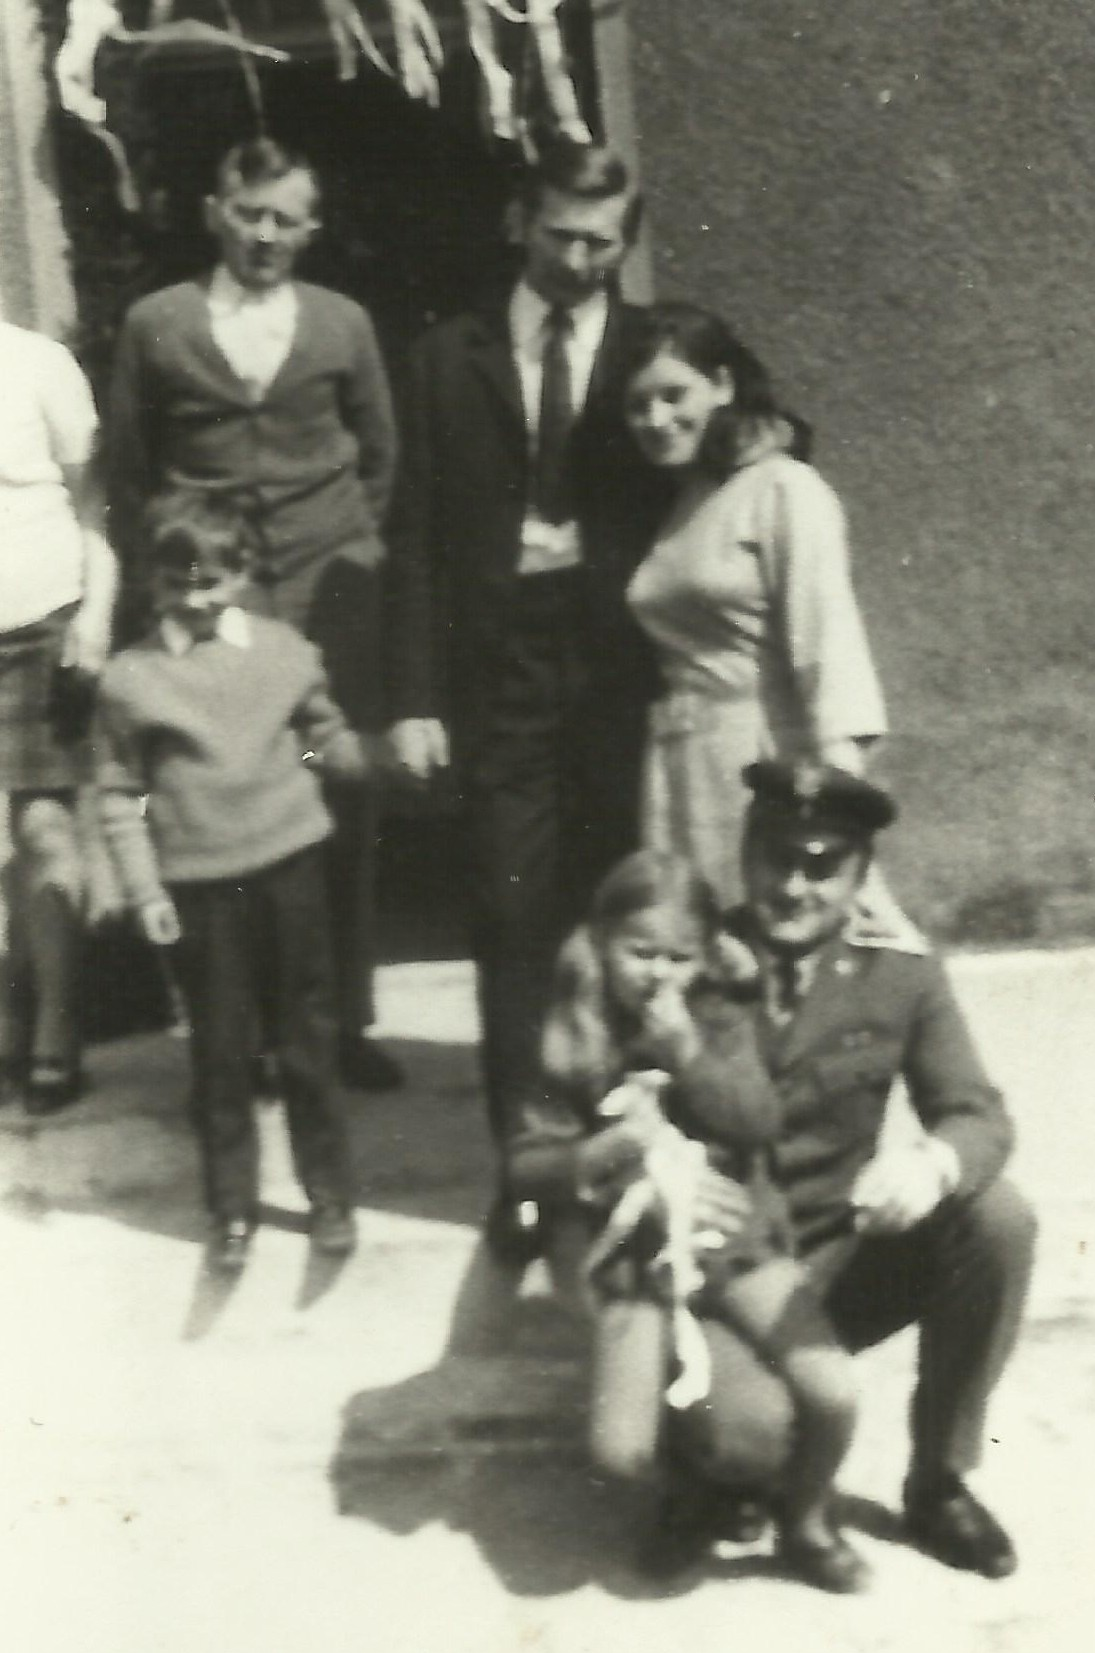
\includegraphics[width=0.4\textwidth]{zdjecia/boleslaw_kurek_z_synem_i_zieciem.jpg}
\caption[Bolesław Kurek z synem, synową i zięciem]{Na zdjęciu z tyłu stoją od lewej: Bolesław Kurek, jego syn Grzegorz z żoną Janiną z domu Radosz, trzyma za rękę syna brata Eugeniusza - Jarosława, z przodu zięć Bolesława - Bronisław Kuklis z córką Jolantą.}
\label{rys:boleslaw_kurek_z_synem_i_zieciem}
\end{center}
\end{figure}

Mieli oni pięcioro dzieci. Pierwszy syn żył tylko kilka dni. Następną była córka Irena, która zmarła mając około roku, prawdopodobnie w skutek niewłaściwego pokarmu pochodzącego od koleżanki Bolesławy, która gościła na weselu w Mirowie.
Kolejnymi dziećmi byli: syn Eugeniusz (ur. 12 V 1935 r. w Mirowie), córka Anna (ur. 27 IX 1944~r. w~Mirowie) oraz syn Walenty Grzegorz (ur. 13 II 1949 r. w Mirowie), który został na ojcowiźnie i wybudował tam nowy dom.







\section{Eugeniusz Kurek}

Syn Eugeniusz ożenił się dnia 18 II 1962 r. w Myszkowie z Zofią Nowakowską (ur. 10 II 1942 r. w Myszkowie~-~Ciszówce z ojca Antoniego i matki Eleonory z domu Nowak) i ma z nią dwoje dzieci: syna Jarosława Piotra (ur. 1 VIII 1964 r. w Myszkowie~-~Ciszówce) i córkę Wiolettę Annę (ur. 28 III 1973 r. w~Myszkowie). Jarosław ożenił się dnia 16 IV 1988 r. z Lidią Dryndą (ur. w parafii Mrzygłód) i nie doczekali się potomstwa. Wioletta wyszła za Dariusza Pniaka i ma z nim syna Mateusza. Ich rodzice już nie żyją. Zofia zmarła dnia 2 VII 1983 r., a Eugeniusz po jej śmierci uległ zupełnie chorobie alkoholowej i zmarł opuszczony przez rodzinę dnia 3 XI 1989 r. w Myszkowie.




\section{Anna Kuklis z domu Kurek}

\begin{figure}[!h]
\begin{center}
\includegraphics[width=0.35\textwidth]{zdjecia/slub_jolanty_i_jaroslawa_wylezalkow.jpg}
\caption[Ślub Jolanty Kuklis z Jarosławem Wylężałkiem]{Ślub Jolanty z domu Kuklis (wnuczki Bolesławy) i Jarosława Wylężałków}
\label{rys:slub_jolanty_i_jaroslawa_wylezalkow}
\end{center}
\end{figure}

Anna Kurkówna wyszła dnia 10 X 1965 r. w Niegowie w USC za Bronisława Kuklisa (ur. 1 IX 1942 r.) i ma z nim trzy córki: Jolantę (ur. 15 X 1966 r. w Myszkowie), Dorotę (ur. 27 VIII 1969 r. w Miasteczku Śląskim) oraz najmłodszą Izabelę (ur. 24 X 1973 r. w Lublińcu). Wszystkie trzy wyszły za mąż.

{\color{red}
%TODO
*** Tu zdj. Jolanty i Jarosława Wyleżałków z dziećmi}


Jolanta wyszła za Jarosława Wyleżałka (ur. 20 XI 1966 r.) i ma z nim córkę Aleksandrę (ur. 28 III 1992 r.) oraz syna Szymona (ur. 3 I 1997 r.).

{\color{red}
%TODO
***Tu zdj. Doroty i Romualda Benduchów z córkami}

Dorota wyszła za Romualda Benducha (ur. 27 XI 1969 r.) i ma z nim dwie córki: Wiktorię (ur. 4~VI~1997~r.) i Marię (ur. 10 XII 2001 r.).

{\color{red}
%TODO
***Tu zdj. Izy i Piotra Płonków z córką}

Iza wyszła za Piotra Płonkę (ur. 22 VIII 1973 r. w Tarnowskich Górach) i ma z nim córkę Natalię (ur. 2 I 2001 r.)

Bronisław Kuklis zmarł dnia 4 I 2006 r. w Tarnowskich Górach na zawał serca.




\section{Grzegorz Walenty Kurek}

\begin{figure}[!hb]
\begin{center}
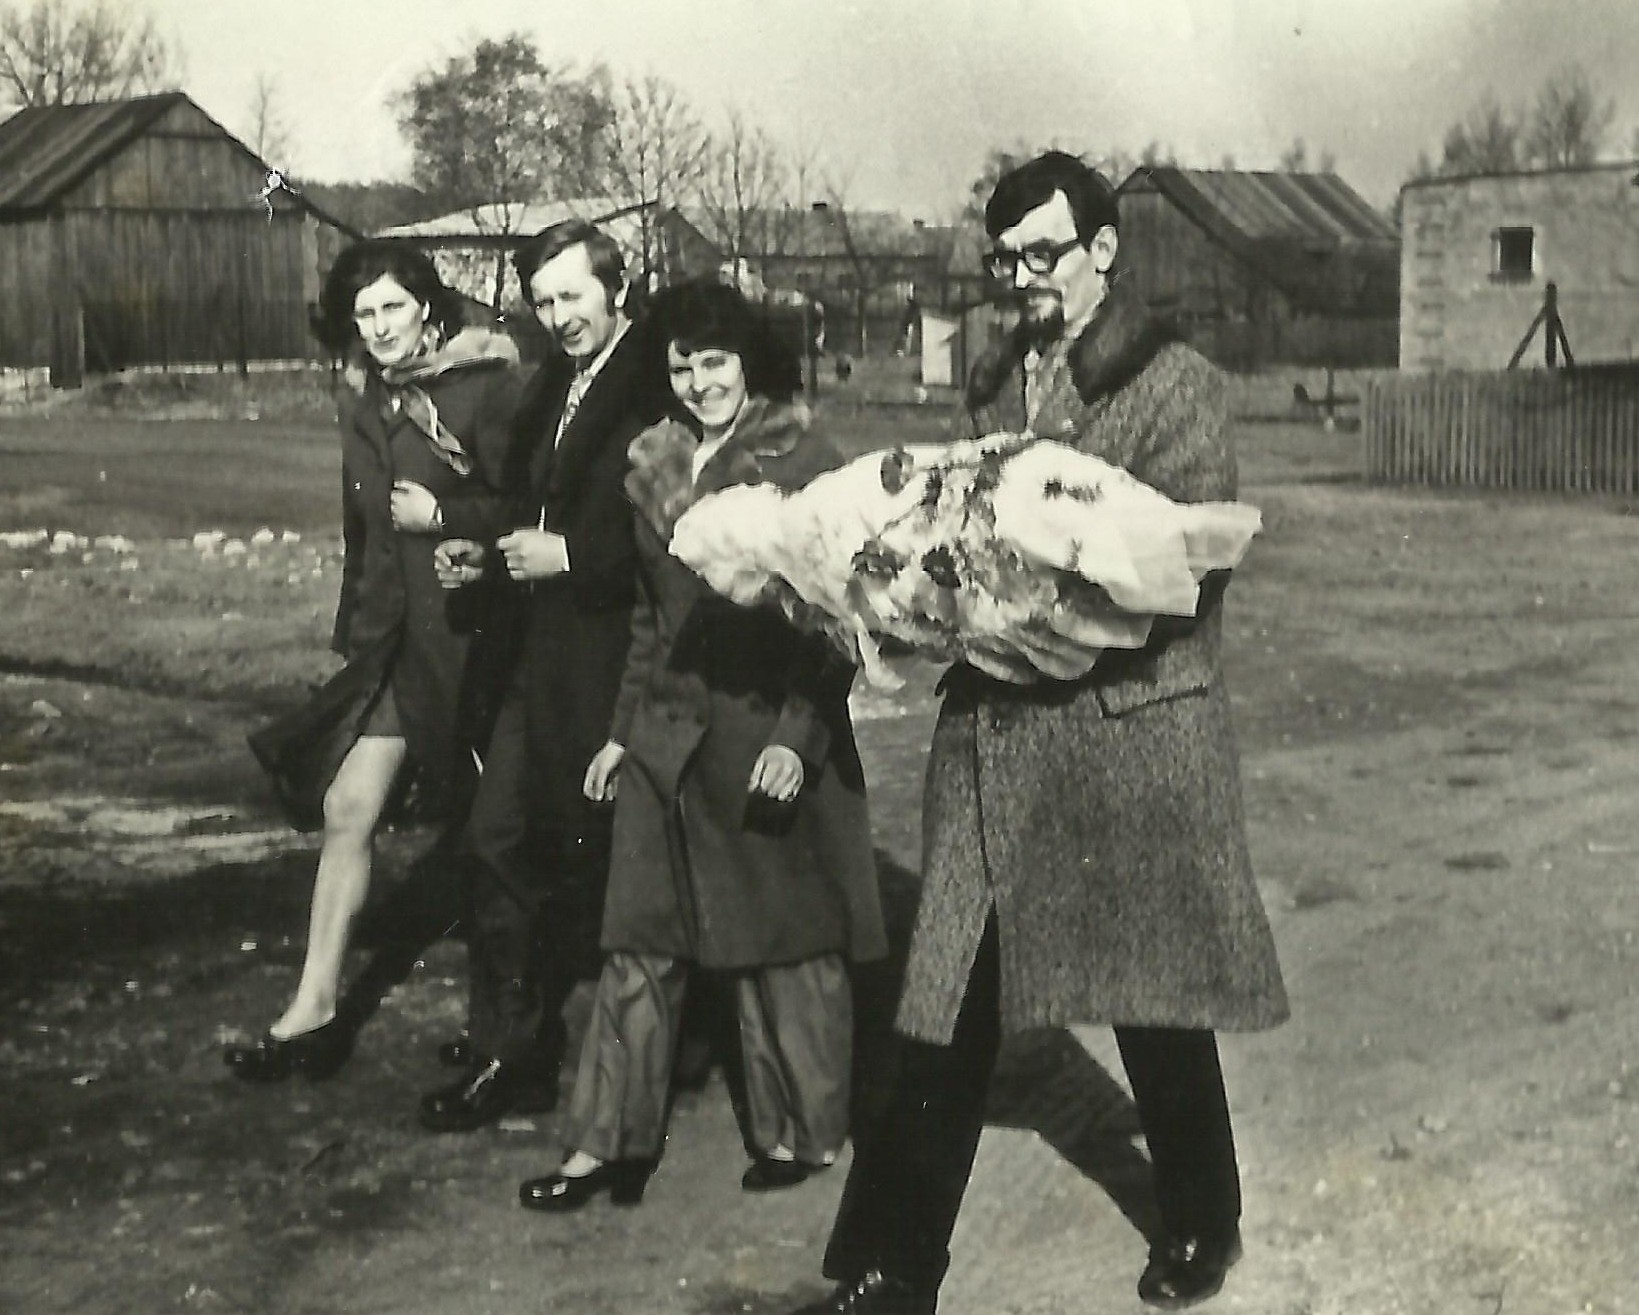
\includegraphics[width=0.5\textwidth]{zdjecia/chrzest_mariusza_kurka.jpg}
\caption[Chrzest św. Mariusza Kurka]{Chrzest św. Mariusza Kurka. Od lewej: Janina i Grzegorz Kurkowie -- rodzice, następnie Barbara Radosz i Czesław Świerczyński -- chrzestni}
\label{rys:chrzest_mariusza_kurka}
\end{center}
\end{figure}

\begin{figure}[!h]
\begin{center}
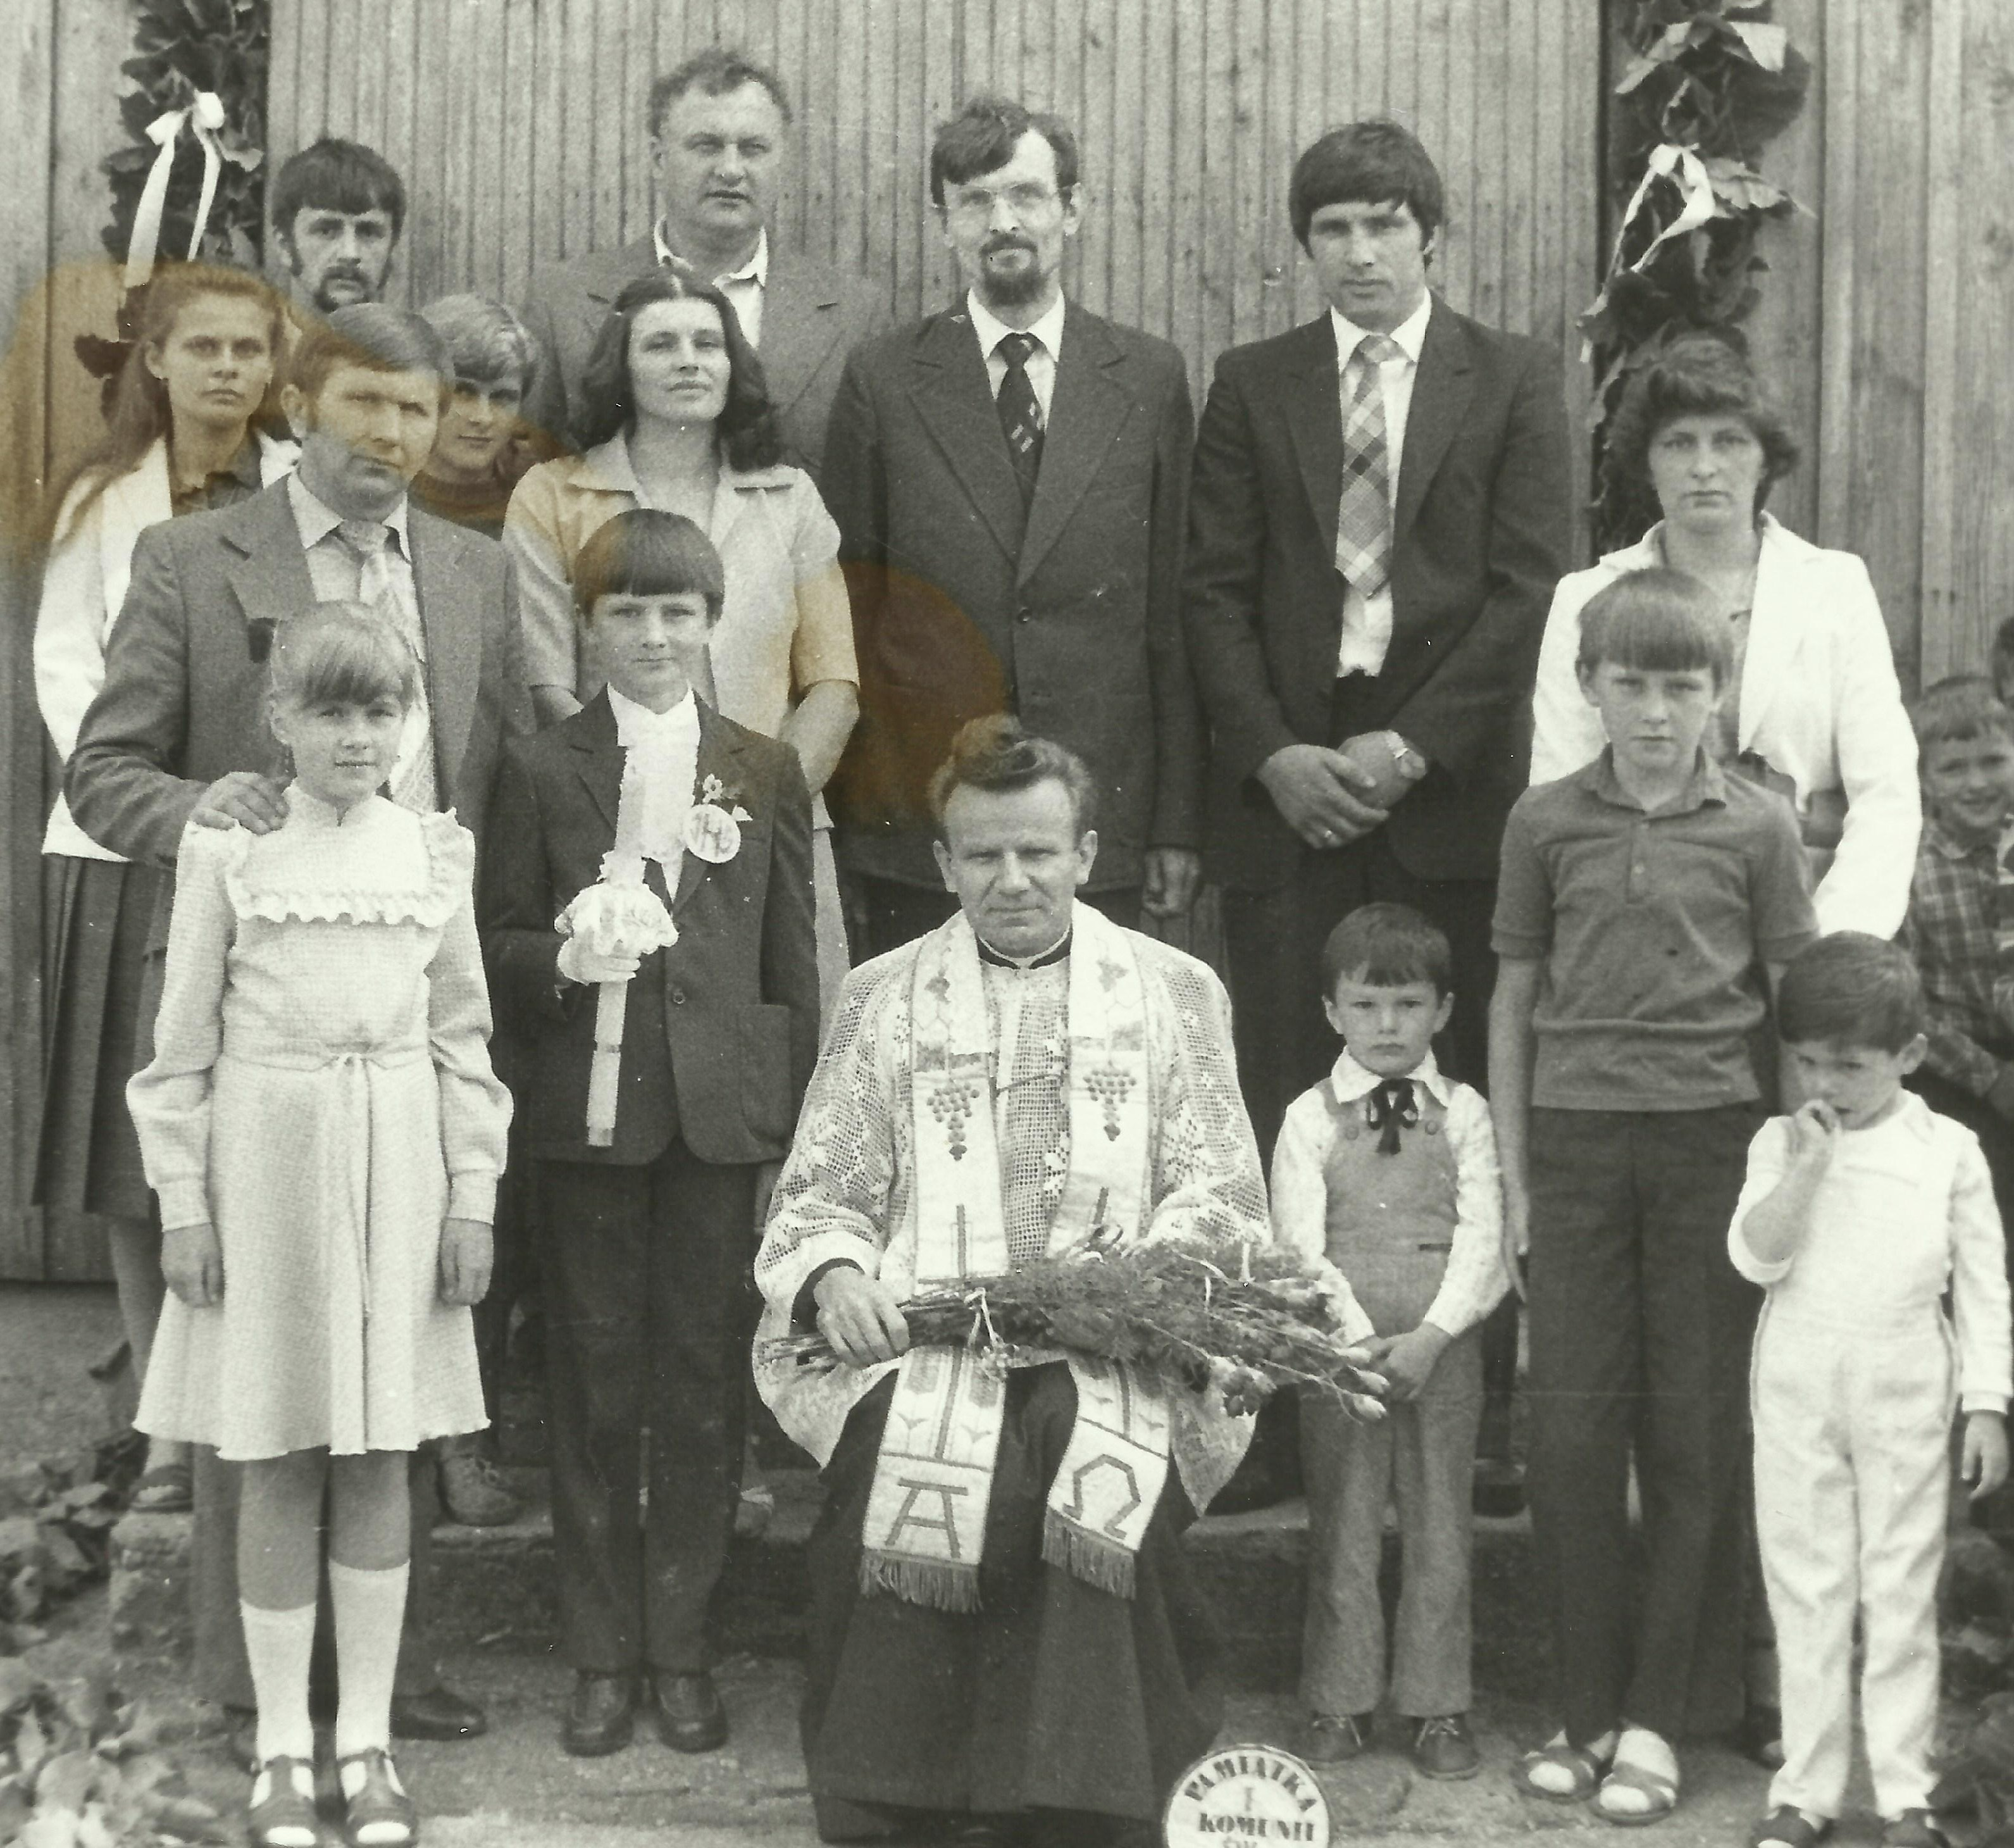
\includegraphics[width=0.8\textwidth]{zdjecia/pierwsza_komunia_mariusza_kurka.jpg}
\caption[Pierwsza komunia św. Mariusza Kurka]{Pierwsza komunia św. Mariusza Kurka, wnuczka Bolesławy Kurek z domu Głąb. Od lewej w trzecim rzędzie: Zbigniew Kasprzyk, mąż Barbary Radosz Kasprzyk, Bronisław Kuklis, Czesław Świerczyński -- chrzestny Mariusza, Sylwester Radosz obok siostry Janiny Kurek, w drugim rzędzie od lewej Jolanta Kuklis, Dorota Kuklis, Barbara Radosz-Kasprzyk, Grzegorz Kurek, przed nim Iza Kuklis, obok Mariusz Kurek, ks. Florian Nejman, obok księdza Artur Kasprzyk, Arek Kurek, Rafał Radosz.}
\label{rys:pierwsza_komunia_mariusza_kurka}
\end{center}
\end{figure}

\begin{figure}[!h]
\begin{center}
\includegraphics[width=0.7\textwidth]{zdjecia/grzegorz_kurek_z_synami.jpg}
\caption[Grzegorz Kurek z synami]{Grzegorz Kurek z synami: z lewej Mariuszem i z prawej Arkadiuszem}
\label{rys:grzegorz_kurek_z_synami}
\end{center}
\end{figure}

Najmłodszy syn Bolesławy i Bolesława Kurków -- Walenty Grzegorz Kurek ożenił się dnia 30 IV 1972~r. w Niegowie z Janiną Radosz (ur. 11 V 1952 r. w Mirowie z ojca Jana i matki Kazimiery z domu Gurbała) i ma z nią trzech synów: Arkadiusza Piotra (ur. 18 X 1972 r. w Żarkach), Mariusza Grzegorza (ur. 17 II 1974 r. w Żarkach) oraz najmłodszego Przemysława Jana (ur. 4 V 1984 r. w Bytomiu).


\begin{figure}[!h]
\begin{center}
\includegraphics[width=0.4\textwidth]{zdjecia/komunia_mateusza_kurka.jpg}
\caption[I Komunia św, Mateusza Kurka]{I Komunia św, Mateusza Kurka, syna Arkadiusza. Od lewej: Arkadiusz i Marzena Kurkowie -- rodzice, dalej matka chrzestna i Mariusz Kurek -- chrzestny, obok Mateusza jego młodszy brat Kuba}
\label{rys:komunia_mateusza_kurka}
\end{center}
\end{figure}

Dwaj starsi bracia pożenili się. Arkadiusz dnia 23 IX 1995 r. we Wróblewie (k. Sieradza) z Marzeną Zdunek (ur. 25 VIII 1973 r. w Sieradzu z ojca Janusza i matki Zdzisławy z domu Namysł), a Mariusz 30 XII 2007~r. w Podlesiu (k. Koniecpola) z Iwoną Kłopot (ur. 15 II 1975~r. w Częstochowie z ojca Kazimierza i matki Danuty z domu Siedmilat). Arkadiusz i Marzena Kurkowie doczekali się dwóch synów: Mateusza (ur. 8 X 1996~r. w Sieradzu) i Jakuba (ur. 23 XII 1999~r. w Łodzi). Mariusz i Iwona Kurkowie mają syna Huberta (ur. 21 V 2008~r. w Częstochowie). Wybudowali oni dom w Mirowie na działce w pobliżu domu autora niniejszej historii rodowej Głąbów, gdzie mają zamiar wkrótce zamieszkać.
%TODOzdj. domu Mariusza i Iwony Kurków w obecnym sdtanie.

\begin{figure}[!h]
\begin{center}
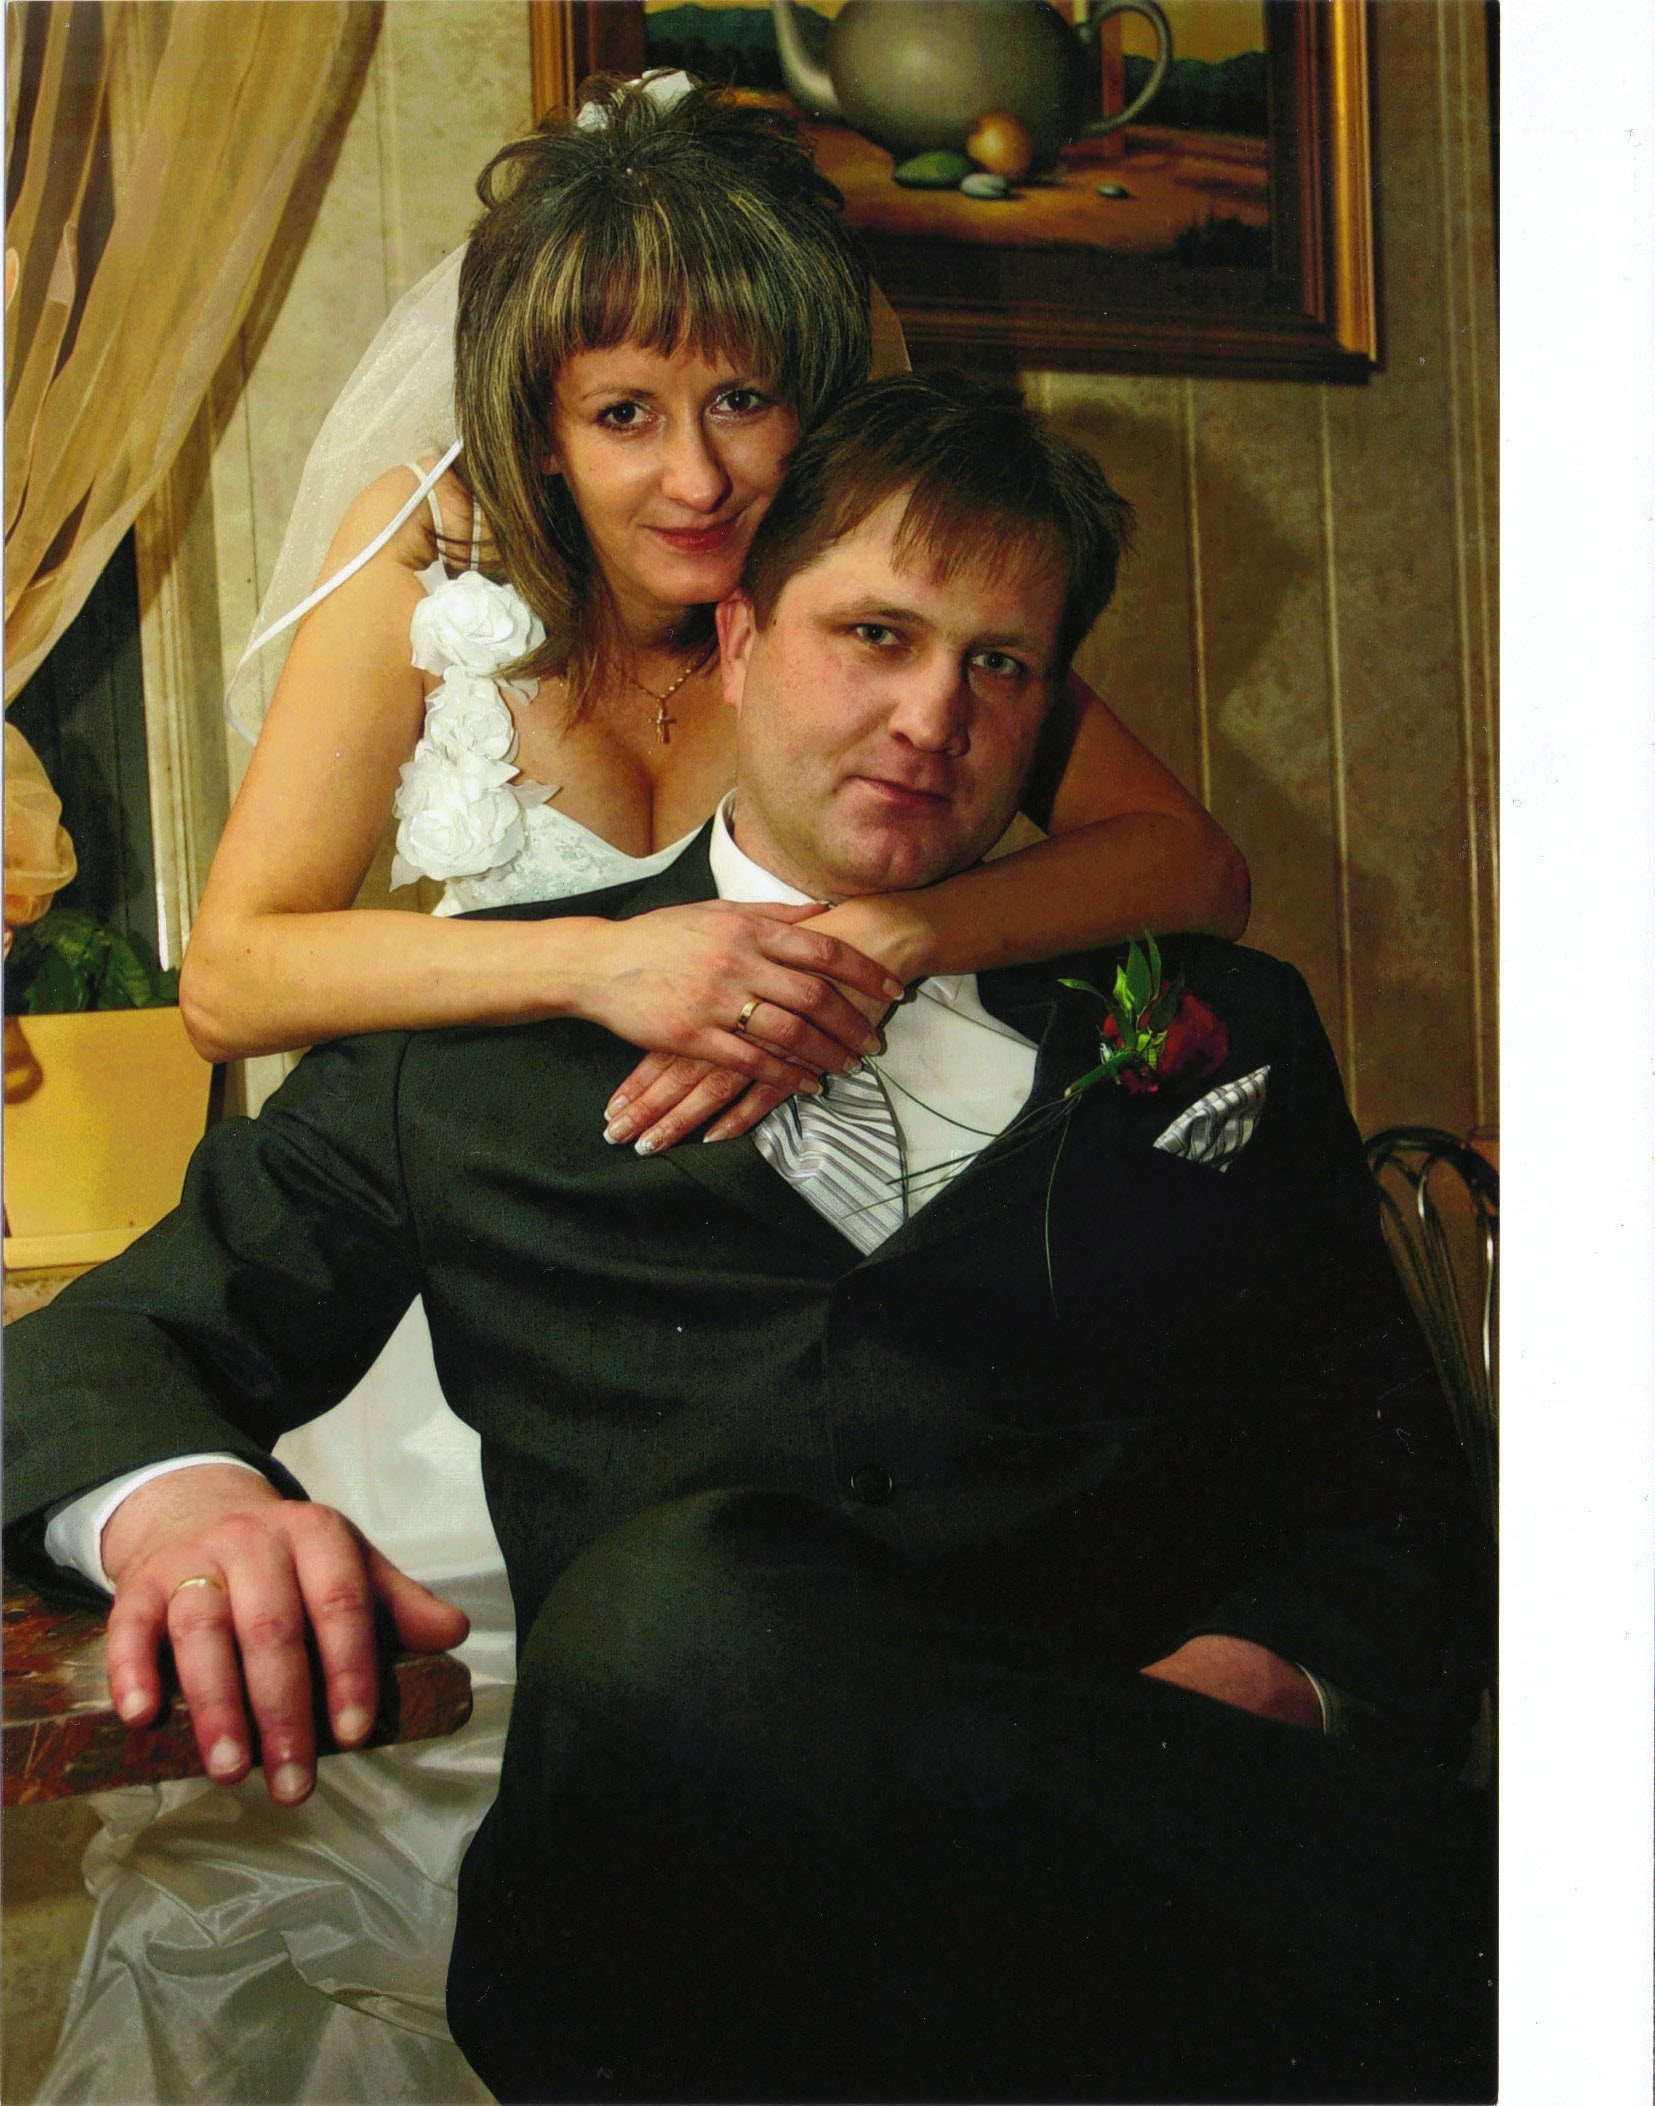
\includegraphics[width=0.5\textwidth]{zdjecia/mariusz_i_iwona_kurek.jpg}
\caption[Ślub Mariusza Kurka z Iwoną Kłopot]{Ślub Mariusza Kurka -- wnuczka Bolesławy Kurek z domu Głąb i Iwony Kłopot}
\label{rys:mariusz_i_iwona_kurek}
\end{center}
\end{figure}

\begin{figure}[!h]
\begin{center}
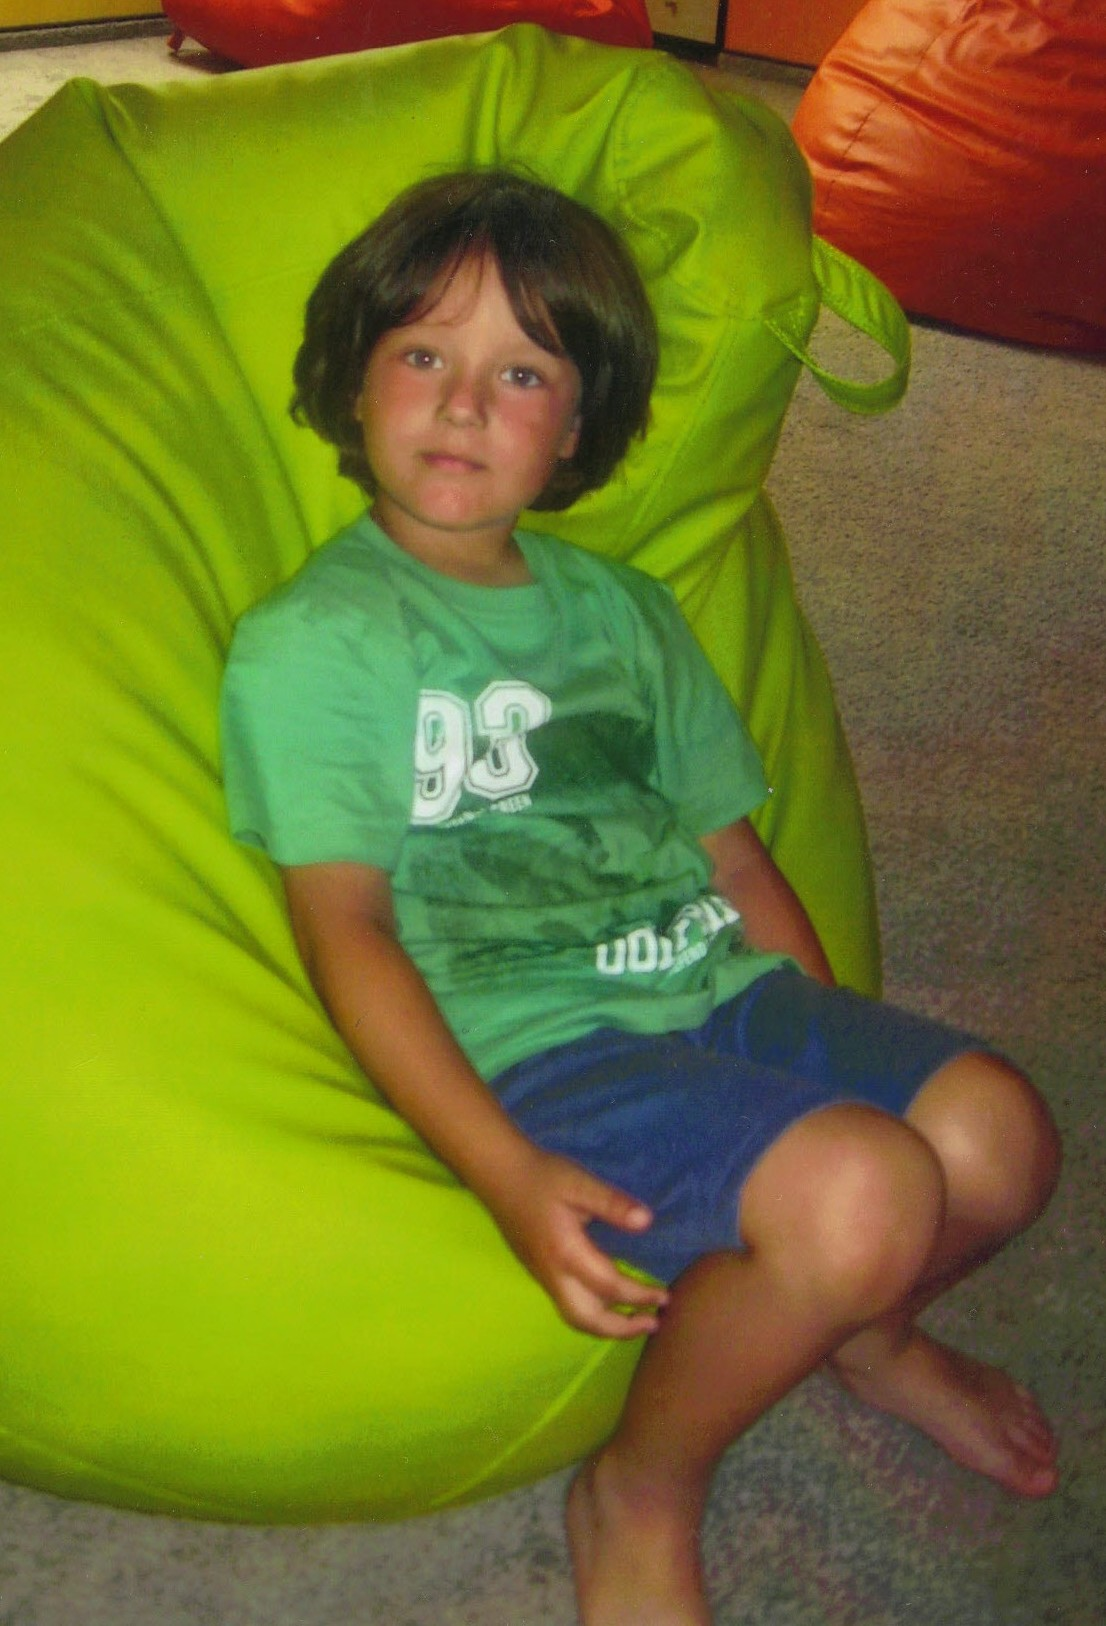
\includegraphics[width=0.4\textwidth]{zdjecia/hubert_kurek.jpg}
\caption[Hubert Kurek]{Hubert Kurek -- prawnuczek Bolesławy Kurek z domu Głąb}
\label{rys:hubert_kurek}
\end{center}
\end{figure}

Bolesław Kurek zmarł 12 II 1973 r. w Mirowie, a jego małżonka Bolesława zmarła w 33 lata później, tj. 17~I~2006~r. także w Mirowie. Miała 98 lat.



